
%% bare_conf_compsoc.tex
%% V1.4b
%% 2015/08/26
%% by Michael Shell
%% See:
%% http://www.michaelshell.org/
%% for current contact information.
%%
%% This is a skeleton file demonstrating the use of IEEEtran.cls
%% (requires IEEEtran.cls version 1.8b or later) with an IEEE Computer
%% Society conference paper.
%%
%% Support sites:
%% http://www.michaelshell.org/tex/ieeetran/
%% http://www.ctan.org/pkg/ieeetran
%% and
%% http://www.ieee.org/

%%*************************************************************************
%% Legal Notice:
%% This code is offered as-is without any warranty either expressed or
%% implied; without even the implied warranty of MERCHANTABILITY or
%% FITNESS FOR A PARTICULAR PURPOSE! 
%% User assumes all risk.
%% In no event shall the IEEE or any contributor to this code be liable for
%% any damages or losses, including, but not limited to, incidental,
%% consequential, or any other damages, resulting from the use or misuse
%% of any information contained here.
%%
%% All comments are the opinions of their respective authors and are not
%% necessarily endorsed by the IEEE.
%%
%% This work is distributed under the LaTeX Project Public License (LPPL)
%% ( http://www.latex-project.org/ ) version 1.3, and may be freely used,
%% distributed and modified. A copy of the LPPL, version 1.3, is included
%% in the base LaTeX documentation of all distributions of LaTeX released
%% 2003/12/01 or later.
%% Retain all contribution notices and credits.
%% ** Modified files should be clearly indicated as such, including  **
%% ** renaming them and changing author support contact information. **
%%*************************************************************************


% *** Authors should verify (and, if needed, correct) their LaTeX system  ***
% *** with the testflow diagnostic prior to trusting their LaTeX platform ***
% *** with production work. The IEEE's font choices and paper sizes can   ***
% *** trigger bugs that do not appear when using other class files.       ***                          ***
% The testflow support page is at:
% http://www.michaelshell.org/tex/testflow/

\documentclass[10pt, conference, compsocconf]{IEEEtran}
% Some/most Computer Society conferences require the compsoc mode option,
% but others may want the standard conference format.
%
% If IEEEtran.cls has not been installed into the LaTeX system files,
% manually specify the path to it like:
% \documentclass[conference,compsoc]{../sty/IEEEtran}

\usepackage{hyperref}

% PDF Settings
\hypersetup{
%    bookmarks=true,         % show bookmarks bar?
%    unicode=false,          % non-Latin characters in Acrobat�s bookmarks
%    pdftoolbar=true,        % show Acrobat's toolbar?
%    pdfmenubar=true,        % show Acrobat's menu?
%    pdffitwindow=false,     % window fit to page when opened
%    pdfstartview={FitH},    % fits the width of the page to the window
    pdftitle={DataWarp Transparent Cache: Implementation, Challenges, and Early Experience},    % title
    pdfauthor={David Paul, Benjamin Landsteiner},     % author
    pdfsubject={DataWarp},   % subject of the document
%    pdfcreator={Creator},   % creator of the document
%    pdfproducer={Producer}, % producer of the document
    pdfkeywords={SSD, Cache, DataWarp, Experience, Lessons, Filesystems}, % list of keywords
%    pdfnewwindow=true,      % links in new window
%    colorlinks=false,       % false: boxed links; true: colored links
%    linkcolor=red,          % color of internal links
%    citecolor=green,        % color of links to bibliography
%    filecolor=magenta,      % color of file links
%    urlcolor=cyan           % color of external links
}


% Some very useful LaTeX packages include:
% (uncomment the ones you want to load)


% *** MISC UTILITY PACKAGES ***
%
%\usepackage{ifpdf}
% Heiko Oberdiek's ifpdf.sty is very useful if you need conditional
% compilation based on whether the output is pdf or dvi.
% usage:
% \ifpdf
%   % pdf code
% \else
%   % dvi code
% \fi
% The latest version of ifpdf.sty can be obtained from:
% http://www.ctan.org/pkg/ifpdf
% Also, note that IEEEtran.cls V1.7 and later provides a builtin
% \ifCLASSINFOpdf conditional that works the same way.
% When switching from latex to pdflatex and vice-versa, the compiler may
% have to be run twice to clear warning/error messages.



% *** CITATION PACKAGES ***
%
\ifCLASSOPTIONcompsoc
  % IEEE Computer Society needs nocompress option
  % requires cite.sty v4.0 or later (November 2003)
  \usepackage[nocompress]{cite}
\else
  % normal IEEE
  \usepackage{cite}
\fi
% cite.sty was written by Donald Arseneau
% V1.6 and later of IEEEtran pre-defines the format of the cite.sty package
% \cite{} output to follow that of the IEEE. Loading the cite package will
% result in citation numbers being automatically sorted and properly
% "compressed/ranged". e.g., [1], [9], [2], [7], [5], [6] without using
% cite.sty will become [1], [2], [5]--[7], [9] using cite.sty. cite.sty's
% \cite will automatically add leading space, if needed. Use cite.sty's
% noadjust option (cite.sty V3.8 and later) if you want to turn this off
% such as if a citation ever needs to be enclosed in parenthesis.
% cite.sty is already installed on most LaTeX systems. Be sure and use
% version 5.0 (2009-03-20) and later if using hyperref.sty.
% The latest version can be obtained at:
% http://www.ctan.org/pkg/cite
% The documentation is contained in the cite.sty file itself.
%
% Note that some packages require special options to format as the Computer
% Society requires. In particular, Computer Society  papers do not use
% compressed citation ranges as is done in typical IEEE papers
% (e.g., [1]-[4]). Instead, they list every citation separately in order
% (e.g., [1], [2], [3], [4]). To get the latter we need to load the cite
% package with the nocompress option which is supported by cite.sty v4.0
% and later.





% *** GRAPHICS RELATED PACKAGES ***
%
\ifCLASSINFOpdf
  \usepackage[pdftex]{graphicx}
  % declare the path(s) where your graphic files are
  % \graphicspath{{../pdf/}{../jpeg/}}
  % and their extensions so you won't have to specify these with
  % every instance of \includegraphics
  % \DeclareGraphicsExtensions{.pdf,.jpeg,.png}
\else
  % or other class option (dvipsone, dvipdf, if not using dvips). graphicx
  % will default to the driver specified in the system graphics.cfg if no
  % driver is specified.
  % \usepackage[dvips]{graphicx}
  % declare the path(s) where your graphic files are
  % \graphicspath{{../eps/}}
  % and their extensions so you won't have to specify these with
  % every instance of \includegraphics
  % \DeclareGraphicsExtensions{.eps}
\fi
% This has to be after graphicx???
\usepackage{pgfplots}
\pgfplotsset{compat=1.13}
\usepgfplotslibrary{external}
\tikzexternalize

% graphicx was written by David Carlisle and Sebastian Rahtz. It is
% required if you want graphics, photos, etc. graphicx.sty is already
% installed on most LaTeX systems. The latest version and documentation
% can be obtained at: 
% http://www.ctan.org/pkg/graphicx
% Another good source of documentation is "Using Imported Graphics in
% LaTeX2e" by Keith Reckdahl which can be found at:
% http://www.ctan.org/pkg/epslatex
%
% latex, and pdflatex in dvi mode, support graphics in encapsulated
% postscript (.eps) format. pdflatex in pdf mode supports graphics
% in .pdf, .jpeg, .png and .mps (metapost) formats. Users should ensure
% that all non-photo figures use a vector format (.eps, .pdf, .mps) and
% not a bitmapped formats (.jpeg, .png). The IEEE frowns on bitmapped formats
% which can result in "jaggedy"/blurry rendering of lines and letters as
% well as large increases in file sizes.
%
% You can find documentation about the pdfTeX application at:
% http://www.tug.org/applications/pdftex





% *** MATH PACKAGES ***
%
%\usepackage{amsmath}
% A popular package from the American Mathematical Society that provides
% many useful and powerful commands for dealing with mathematics.
%
% Note that the amsmath package sets \interdisplaylinepenalty to 10000
% thus preventing page breaks from occurring within multiline equations. Use:
%\interdisplaylinepenalty=2500
% after loading amsmath to restore such page breaks as IEEEtran.cls normally
% does. amsmath.sty is already installed on most LaTeX systems. The latest
% version and documentation can be obtained at:
% http://www.ctan.org/pkg/amsmath





% *** SPECIALIZED LIST PACKAGES ***
%
%\usepackage{algorithmic}
% algorithmic.sty was written by Peter Williams and Rogerio Brito.
% This package provides an algorithmic environment fo describing algorithms.
% You can use the algorithmic environment in-text or within a figure
% environment to provide for a floating algorithm. Do NOT use the algorithm
% floating environment provided by algorithm.sty (by the same authors) or
% algorithm2e.sty (by Christophe Fiorio) as the IEEE does not use dedicated
% algorithm float types and packages that provide these will not provide
% correct IEEE style captions. The latest version and documentation of
% algorithmic.sty can be obtained at:
% http://www.ctan.org/pkg/algorithms
% Also of interest may be the (relatively newer and more customizable)
% algorithmicx.sty package by Szasz Janos:
% http://www.ctan.org/pkg/algorithmicx




% *** ALIGNMENT PACKAGES ***
%
%\usepackage{array}
% Frank Mittelbach's and David Carlisle's array.sty patches and improves
% the standard LaTeX2e array and tabular environments to provide better
% appearance and additional user controls. As the default LaTeX2e table
% generation code is lacking to the point of almost being broken with
% respect to the quality of the end results, all users are strongly
% advised to use an enhanced (at the very least that provided by array.sty)
% set of table tools. array.sty is already installed on most systems. The
% latest version and documentation can be obtained at:
% http://www.ctan.org/pkg/array


% IEEEtran contains the IEEEeqnarray family of commands that can be used to
% generate multiline equations as well as matrices, tables, etc., of high
% quality.




% *** SUBFIGURE PACKAGES ***
\ifCLASSOPTIONcompsoc
  \usepackage[caption=false,font=footnotesize,labelfont=sf,textfont=sf]{subfig}
\else
  \usepackage[caption=false,font=footnotesize]{subfig}
\fi
% subfig.sty, written by Steven Douglas Cochran, is the modern replacement
% for subfigure.sty, the latter of which is no longer maintained and is
% incompatible with some LaTeX packages including fixltx2e. However,
% subfig.sty requires and automatically loads Axel Sommerfeldt's caption.sty
% which will override IEEEtran.cls' handling of captions and this will result
% in non-IEEE style figure/table captions. To prevent this problem, be sure
% and invoke subfig.sty's "caption=false" package option (available since
% subfig.sty version 1.3, 2005/06/28) as this is will preserve IEEEtran.cls
% handling of captions.
% Note that the Computer Society format requires a sans serif font rather
% than the serif font used in traditional IEEE formatting and thus the need
% to invoke different subfig.sty package options depending on whether
% compsoc mode has been enabled.
%
% The latest version and documentation of subfig.sty can be obtained at:
% http://www.ctan.org/pkg/subfig




% *** FLOAT PACKAGES ***
%
%\usepackage{fixltx2e}
% fixltx2e, the successor to the earlier fix2col.sty, was written by
% Frank Mittelbach and David Carlisle. This package corrects a few problems
% in the LaTeX2e kernel, the most notable of which is that in current
% LaTeX2e releases, the ordering of single and double column floats is not
% guaranteed to be preserved. Thus, an unpatched LaTeX2e can allow a
% single column figure to be placed prior to an earlier double column
% figure.
% Be aware that LaTeX2e kernels dated 2015 and later have fixltx2e.sty's
% corrections already built into the system in which case a warning will
% be issued if an attempt is made to load fixltx2e.sty as it is no longer
% needed.
% The latest version and documentation can be found at:
% http://www.ctan.org/pkg/fixltx2e


\usepackage{stfloats}
% stfloats.sty was written by Sigitas Tolusis. This package gives LaTeX2e
% the ability to do double column floats at the bottom of the page as well
% as the top. (e.g., "\begin{figure*}[!b]" is not normally possible in
% LaTeX2e). It also provides a command:
%\fnbelowfloat
% to enable the placement of footnotes below bottom floats (the standard
% LaTeX2e kernel puts them above bottom floats). This is an invasive package
% which rewrites many portions of the LaTeX2e float routines. It may not work
% with other packages that modify the LaTeX2e float routines. The latest
% version and documentation can be obtained at:
% http://www.ctan.org/pkg/stfloats
% Do not use the stfloats baselinefloat ability as the IEEE does not allow
% \baselineskip to stretch. Authors submitting work to the IEEE should note
% that the IEEE rarely uses double column equations and that authors should try
% to avoid such use. Do not be tempted to use the cuted.sty or midfloat.sty
% packages (also by Sigitas Tolusis) as the IEEE does not format its papers in
% such ways.
% Do not attempt to use stfloats with fixltx2e as they are incompatible.
% Instead, use Morten Hogholm'a dblfloatfix which combines the features
% of both fixltx2e and stfloats:
%
% \usepackage{dblfloatfix}
% The latest version can be found at:
% http://www.ctan.org/pkg/dblfloatfix




% *** PDF, URL AND HYPERLINK PACKAGES ***
%
\usepackage{url}
% url.sty was written by Donald Arseneau. It provides better support for
% handling and breaking URLs. url.sty is already installed on most LaTeX
% systems. The latest version and documentation can be obtained at:
% http://www.ctan.org/pkg/url
% Basically, \url{my_url_here}.

\usepackage{xcolor}
\usepackage[most]{tcolorbox}

\lstset{
basicstyle=\ttfamily,
}


% *** Do not adjust lengths that control margins, column widths, etc. ***
% *** Do not use packages that alter fonts (such as pslatex).         ***
% There should be no need to do such things with IEEEtran.cls V1.6 and later.
% (Unless specifically asked to do so by the journal or conference you plan
% to submit to, of course. )


% correct bad hyphenation here
\hyphenation{Data-Warp}


\begin{document}
%
% paper title
% Titles are generally capitalized except for words such as a, an, and, as,
% at, but, by, for, in, nor, of, on, or, the, to and up, which are usually
% not capitalized unless they are the first or last word of the title.
% Linebreaks \\ can be used within to get better formatting as desired.
% Do not put math or special symbols in the title.
\title{DataWarp Transparent Cache: Implementation, Challenges, and Early Experience}


% author names and affiliations
% use a multiple column layout for up to three different
% affiliations
%\author{\IEEEauthorblockN{Michael Shell}
%\IEEEauthorblockA{School of Electrical and\\Computer Engineering\\
%Georgia Institute of Technology\\
%Atlanta, Georgia 30332--0250\\
%Email: http://www.michaelshell.org/contact.html}
%\and
%\IEEEauthorblockN{Homer Simpson}
%\IEEEauthorblockA{Twentieth Century Fox\\
%Springfield, USA\\
%Email: homer@thesimpsons.com}
%\and
%\IEEEauthorblockN{James Kirk\\ and Montgomery Scott}
%\IEEEauthorblockA{Starfleet Academy\\
%San Francisco, California 96678-2391\\
%Telephone: (800) 555--1212\\
%Fax: (888) 555--1212}}

% conference papers do not typically use \thanks and this command
% is locked out in conference mode. If really needed, such as for
% the acknowledgment of grants, issue a \IEEEoverridecommandlockouts
% after \documentclass

% for over three affiliations, or if they all won't fit within the width
% of the page (and note that there is less available width in this regard for
% compsoc conferences compared to traditional conferences), use this
% alternative format:
% 
\author{\IEEEauthorblockN{David Paul\IEEEauthorrefmark{1}, 
Benjamin Landsteiner\IEEEauthorrefmark{2}}
\IEEEauthorblockA{\IEEEauthorrefmark{1}Lawrence Berkeley National Laboratory\\
National Energy Research Scientific Computing Center, Berkeley, CA  94720\\
Email: dpaul@lbl.gov}
\IEEEauthorblockA{\IEEEauthorrefmark{2}Cray Inc., Bloomington, MN  55425\\
Email: ben@cray.com}}




% use for special paper notices
%\IEEEspecialpapernotice{(Invited Paper)}




% make the title area
\maketitle

% As a general rule, do not put math, special symbols or citations
% in the abstract
\begin{abstract}
DataWarp accelerates performance by making use of fast SSDs layered between a parallel file system (PFS) and applications. Transparent caching functionality provides a new way to accelerate application performance. By configuring the SSDs as a transparent cache to the PFS, DataWarp enables improved application performance without requiring users to manually manage the copying of their data between the PFS and DataWarp. We provide an overview of the implementation to show how easy it is to get started. We then cover some of the challenges encountered during implementation.  We discuss our early experience on large systems and share performance collected from NERSC's Cori supercomputer.  We also discuss future work opportunities.
\end{abstract}

\begin{IEEEkeywords}
Filesystems \& I/O, DataWarp, SSD
\end{IEEEkeywords}



% For peer review papers, you can put extra information on the cover
% page as needed:
% \ifCLASSOPTIONpeerreview
% \begin{center} \bfseries EDICS Category: 3-BBND \end{center}
% \fi
%
% For peerreview papers, this IEEEtran command inserts a page break and
% creates the second title. It will be ignored for other modes.
\IEEEpeerreviewmaketitle



\section{Introduction}

Users are attracted to supercomputing platforms because they help solve their problems faster or cheaper than alternatives.  As supercomputers improve, the benefits they provide increase.  Advancements in supercomputing technology are not uniform, and the bottlenecks that emerge can limit a system's and user's potential.  The imbalance between compute and IO performance is one area that has seen focused interest.

There are numerous proposals and deployed solutions that aim to alleviate the disparity in performance between computation and IO.  Compression techniques consume some amount of excess computation and latency for increased effective bandwidth.  Data caching increases bandwidth and decreases latency.  On Cray systems, a recent example of a data cache is the on-node DVS client-side cache~\cite{dvs_client_cache}.  On ClusterStor, the NXD flash accelerator improves performance for small IO headed towards spinning disk~\cite{nxd}.  DDN's IME solution has similar goals~\cite{ddn_ime}.

DataWarp is another solution for accelerating IO performance~\cite{cug_arch} that makes use of data caching techniques.  Instead of having one shared data path for all users on a system, DataWarp can dynamically configure, prepare, and manage new data paths specific to a user's job.  Since user IO requirements and properties vary, a personalized data path using the best available hardware and software can perform better.  Integration with workload managers means that the sometimes critical SSD hardware resource can be shared fairly amongst a system's users.  The scratch data path for DataWarp has been available for some time now with several published success stories~\cite{cug_wahid},~\cite{7836560}.

DataWarp transparent caching introduces a new data path for users to choose.  Using the new data path is easier than the scratch data path because migration of data between the parallel filesystem and DataWarp SSD hardware happens transparently and automatically.  Application performance is improved since data intended for the parallel filesystem is first placed on to a write-back cache backed by SSDs.  We present an overview of the implementation, including the user interface, data path, and orchestration layers in Section~\ref{sec_imp}.  In Section~\ref{sec_chal} we discuss some challenges encountered during the implementation.  We discuss our early experience with transparent caching in Section~\ref{sec_ee}.  We conclude and summarize in Section~\ref{sec_conc}.


\section{Implementation\label{sec_imp}}
DataWarp Transparent Cache functionality extends existing DataWarp infrastructure~\cite{cug_arch}.  With existing DataWarp, users request its functionality with \texttt{\#DW} directives placed alongside workload manager directives in batch job script files.  By the time the job script is executing, the allocated compute environment has been configured to access the requested SSD-backed DataWarp functionality.  By tailoring the hardware and software environment optimal to the job's needs, IO performance is improved and job execution time is reduced.

The configuration steps performed depend on what the user has requested.  Those steps may involve creating a storage allocation across many DataWarp nodes, instantiating a new DataWarp scratch filesystem, allocating swap files, or transferring data from the primary parallel filesystem to the DataWarp scratch filesystem.  Just after compute node allocation but before batch job script execution the filesystem or swap files are made accessible to the job's compute nodes.

For the most part, cleaning up happens in reverse.  Filesystem mounts and swap files are removed from the compute nodes.  Important data is copied from the DataWarp scratch filesystem to the parallel filesystem.  The storage allocation is removed and the SSD space is immediately available to new users.

Users can request a DataWarp transparent cache to transparently and automatically accelerate IO to a parallel filesystem.  This is in contrast to DataWarp scratch environments which requires users to manage all data exchange between it and a parallel filesystem.  A workload manager (WLM) and the DataWarp Service (DWS) software work together to orchestrate the setup and teardown required for the transparent cache data path.

\subsection{User Interface}

The primary way users interact with all variants of DataWarp is through \texttt{\#DW} batch job script directives placed alongside other workload manager directives for compute resources, and environment variables injected in to the batch job script execution process.  For transparent cache, the \texttt{\#DW~jobdw} command is extended to allow users to request it.  There are four mandatory parameters:
\begin{enumerate}
\item \textbf{type=cache} Requests a transparent caching environment
\item \textbf{access\_mode=striped} Requests files be striped across the entire DataWarp allocation (i.e. over multiple servers)
\item \textbf{capacity=100TiB} Specifies the minimum size of the allocation (100TiB in this example)
\item \textbf{pfs=/pfs/path} Specifies which parallel filesystem path DataWarp will transparently accelerate (\texttt{/pfs/path} in this example)
\end{enumerate}
When the batch job script executes, rather than access files under \texttt{/pfs/path}, applications can access the same files at the path defined in \texttt{\$DW\_JOB\_STRIPED\_CACHE} and the DataWarp transparent cache will work to accelerate IO operations.

The \texttt{access\_mode=striped} combination can take two additional configuration options.  These are specified enclosed in parenthesis and appended to the end:
\begin{enumerate}
\item \textbf{MFS=1GiB} Maximum File Size (1GiB in this example)
\item \textbf{client\_cache} Request use of DVS client-side caching on compute nodes when using transparent caching~\cite{dvs_client_cache}
\end{enumerate}

The Maximum File Size configuration option is for helping stop errant IO activity.  Since some of the hardware used by DataWarp are SSDs, and SSDs have a limited write capacity, DataWarp allows users to specify what types of IO activity may signify unintentional excessive usage.  For transparent caching, a user may additionally specify two optional parameters to control how much data can be written to the SSDs in any length of time.  These options have also been available to scratch environments.
\begin{enumerate}
\item \textbf{write\_window\_multiplier=5} Multiplier on capacity for amount allowed to be written (5 in this example)
\item \textbf{write\_window\_length=43200} Number of seconds before a write is no longer considered in calculating excessive usage (43200, or half a day, in this example)
\end{enumerate}
By default, if a user does not specify these two parameters, their job is limited to 10 times the allocation size in writes per 86,400 seconds (1 day).

\begin{figure*}
\small
\begin{tcblisting}{listing only}
#!/bin/bash
#SBATCH --ntasks 3200

export JOBDIR=/lus/global/my_jobdir
srun -n 3200 a.out
\end{tcblisting}
\caption{Example Slurm job script with no DataWarp integration.  \texttt{\$JOBDIR} points to a path on lustre, so \texttt{a.out}'s IO interacts with lustre directly\label{slurm_job_example}}
\end{figure*}

An example Slurm batch job script with no DataWarp integration can be seen in \figurename~\ref{slurm_job_example}.  This basic job script shows an \texttt{a.out} that uses the path specified at \texttt{\$JOBDIR} for IO performed during the job.  In \figurename~\ref{tc_job_example}, the script has been modified to request a 100TiB transparent cache of the parallel filesystem \texttt{/lus/global}.  The path specified at \texttt{\$JOBDIR} has been altered to specify use of the transparent cache.  When \texttt{a.out} now runs, its IO now passes through the transparent cache rather than straight to lustre.  After either job completes, the contents of \texttt{/lus/global/my\_jobdir} are the same.  \figurename~\ref{tc_job_example_knobby} shows an example with the optional settings supplied, and using \texttt{\#DW} line continuation support.

\begin{figure*}
\small
\begin{tcblisting}{listing only}
#!/bin/sh
#SBATCH --ntasks 3200
#DW jobdw type=cache access_mode=striped pfs=/lus/global capacity=100TiB

export JOBDIR=$DW_JOB_STRIPED_CACHE/my_jobdir
srun -n 3200 a.out
\end{tcblisting}
\caption{Example Slurm job script requesting access to a 100TiB transparent cache of \texttt{/lus/global}.  \texttt{\$JOBDIR} now points to \texttt{\$DW\_JOB\_STRIPED\_CACHE/my\_jobdir}.  While to \texttt{a.out} the same files are opened, read, or written as in \figurename~\ref{slurm_job_example}, the IO is actually intercepted by the DataWarp transparent cache.\label{tc_job_example}}
\end{figure*}

\begin{figure*}
\small
\begin{tcblisting}{listing only}
#!/bin/sh
#SBATCH --ntasks 3200
#DW jobdw type=cache access_mode=striped(MFS=10GiB,client_cache) pfs=/lus/global \
#DW       capacity=100TiB write_window_multiplier=5 write_window_length=43200

export JOBDIR=$DW_JOB_STRIPED_CACHE/my_jobdir
srun -n 3200 a.out
\end{tcblisting}
\caption{ Slurm job script requesting transparent caching with many optional settings.\label{tc_job_example_knobby}}
\end{figure*}

While each workload manager with DataWarp support includes its own interface for showing users current DataWarp state, the DWS includes the command \texttt{dwstat} for showing current state.  For transparent cache, the \texttt{dwstat configurations} endpoint includes additional entries for each transparent caching setup.  See \figurename~\ref{dwstat_config_cd} for an example.  The primary column of interest is \texttt{backing\_path}, which displays the parallel filesystem path that the transparent cache configuration will work with.  Other information, such as the size and location of the allocations, are found in other unmodified \texttt{dwstat} endpoints like \texttt{dwstat instances}.

\begin{figure*}
\small
\begin{tcblisting}{listing only}
user@host:~> dwstat configurations --cd
conf state inst  type  amode activs backing_path
1775 CA--- 1787 cache stripe      1 /lus/snx12345
1776 CA--- 1788 cache stripe      1 /lus/global
1777 CA--- 1789 cache stripe      1 /lus/snx12345/alice
\end{tcblisting}
\caption{\texttt{dwstat configurations} output.  The \texttt{--cd} option shows additional details on each of the transparent cache configurations.  Three transparent cache configurations are viewable to the user, and each is transparently caching different paths.\label{dwstat_config_cd}}
\end{figure*}

The DWS includes a separate command, \texttt{dwcli}, to allow administrators to modify DataWarp setup and manually create DataWarp environments.  For transparent caching, this type of configuration can be requested.  The same options that a user normally specifies with \texttt{\#DW} directives in batch job scripts appear as options to \texttt{dwcli}.  See \figurename~\ref{dwcli_create_config} for an example that creates a transparent cache configuration on top of the existing instance \texttt{\$instance}.

\begin{figure*}
\small
\begin{tcblisting}{listing only}
user@host:~> dwcli create configuration --instance $instance \
               --type cache --access-mode stripe --backing-path /lus/snx12345
create request for configurations entity with id = 1776 accepted, "dwstat configurations" for status
\end{tcblisting}
\caption{Creating a transparent cache configuration with \texttt{dwcli}.  Transparent cache configurations are linked with an instance, which is an allocation of space.  Instances are linked with a session, which can be though of as a user.\label{dwcli_create_config}}
\end{figure*}

All operations performed by \texttt{dwstat}, \texttt{dwcli}, and available to users via \texttt{\#DW} directives are funneled through a RESTful API exposed by the DWS.  For transparent caching, the \texttt{/dw/v1/configurations/} endpoint has been augmented to support its new options, such as \texttt{backing\_path}.

\subsection{Data Path}

The transparent caching data path is similar to the scratch data path.  The primary difference is in the introduction of a new filesystem, \texttt{dcfs} or data caching filesystem.  The \texttt{dcfs} manages the contents of a buffer placed between a filesystem and a user of that filesystem.  Whereas in the scratch data path the \texttt{dwfs} or DataWarp filesystem writes files to an SSD-backed XFS filesystem, in the transparent cache data path \texttt{dwfs} writes files to the \texttt{dcfs} filesystem.  The transparent caching data path is covered in depth by "DataWarp Transparent Caching Implementation, CUG2018 - Richardson~\cite{cug_tc_fs}, so only an overview will be presented here.  A visual overview of the transparent cache data path can be seen in \figurename~\ref{tcdp}.

\begin{figure*}
\centering
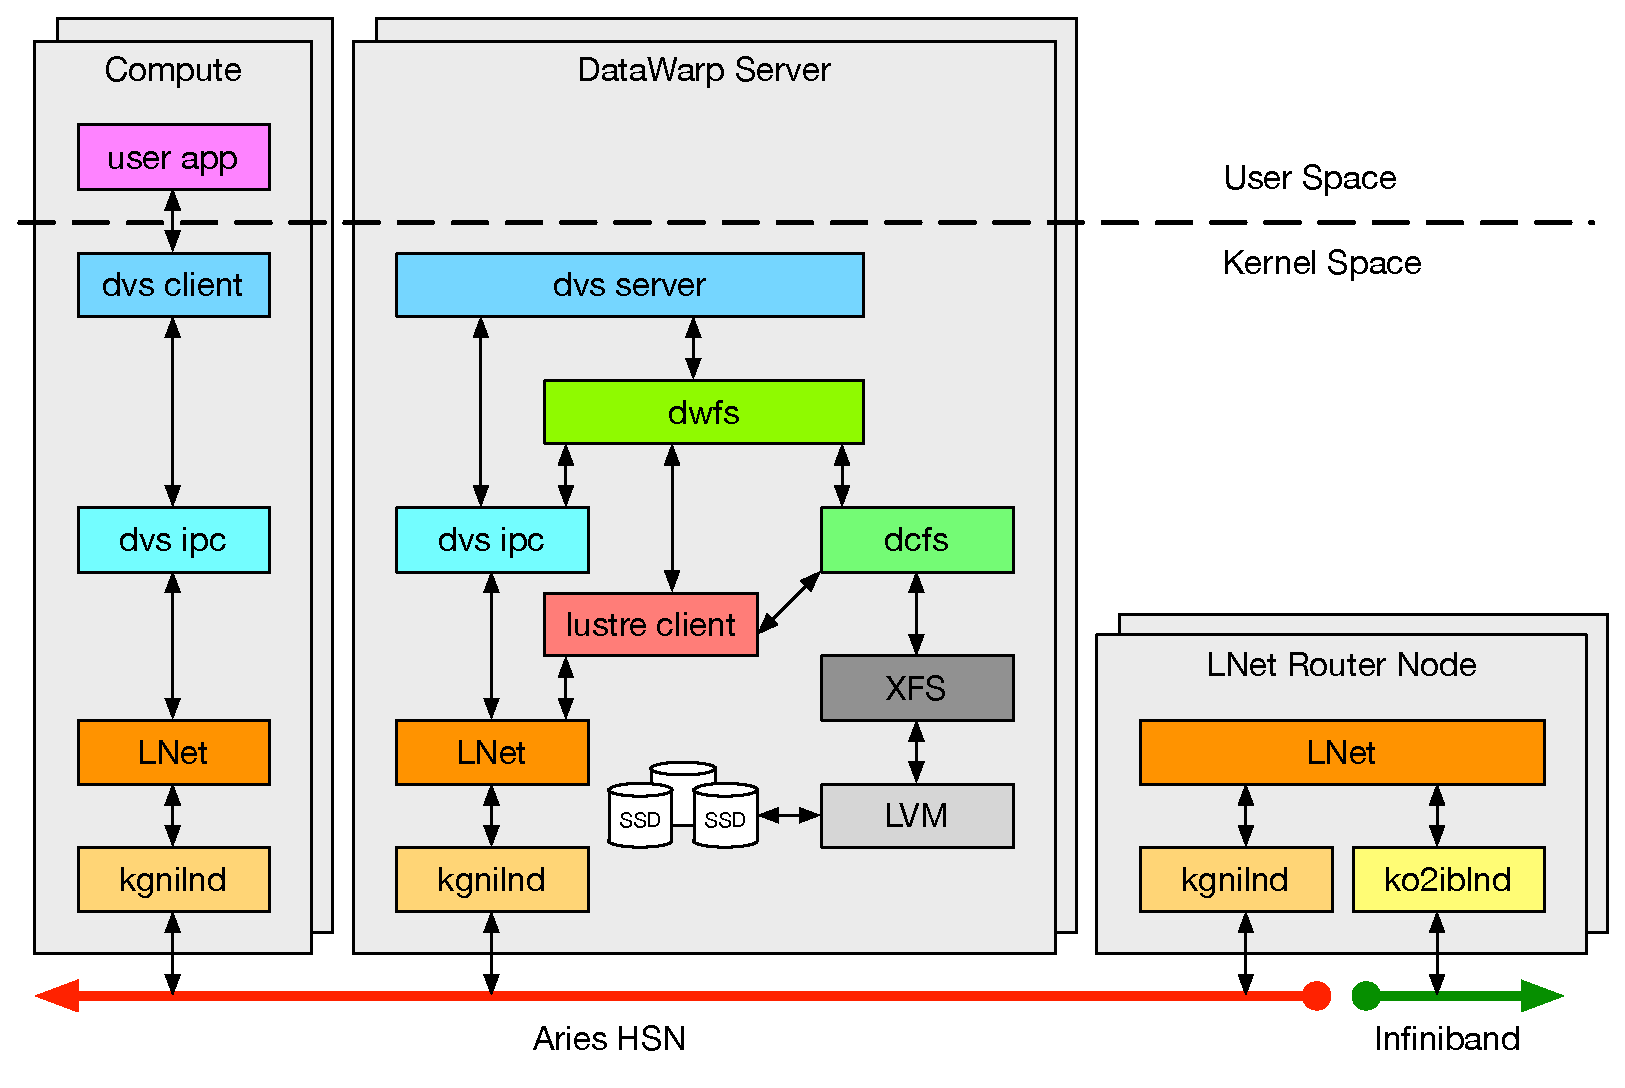
\includegraphics[width=\textwidth]{graphics/tcdp}
\caption{Visual overview of the transparent cache data path.  The \texttt{dcfs} filesystem caches data on to SSD-backed XFS filesystems.\label{tcdp}}
\end{figure*}

On the hardware front, DataWarp server nodes are co-located with compute nodes in Cray XC cabinets.  Compute nodes and DataWarp server nodes are both directly attached to the Aries-based high speed network (HSN).  On the DataWarp server nodes are SSDs with an aggregate bandwidth capacity that matches the capabilities of the Aries NIC.  For a filesystem external to the HSN such as the lustre-based ClusterStor, additional nodes known as LNet router nodes, which are attached to both the Aries HSN and storage network, move IO traffic between lustre clients on the HSN and the external filesystem.

The \texttt{XFS}, \texttt{dcfs}, \texttt{dwfs}, and \texttt{DVS} server reside on DataWarp server nodes.  The \texttt{dcfs} automatically manages file cache data on an \texttt{XFS} filesystem placed on an LVM logical volume striped over the local SSDs.  The \texttt{dcfs} manages files in 1MiB segments internally called extents.  Currently, both cache eviction and dirty data write-back algorithms are file-based LRU (least recently used).  When \texttt{dcfs} processes a \texttt{read()} request, it first sees if the extents are in the cache.  For any cache misses, \texttt{dcfs} performs a copy-up for these extents from the PFS in to the cache.  Once all extents are in the cache, the data requested by the \texttt{read()} is returned.  Processing of a \texttt{write()} is similar, as writes go through a read-modify-write cycle, except for extents wholly overwritten.  Cache eviction and write-back take place automatically after a high watermark threshold of data or dirty data, respectively, is exceeded, and continue until a low watermark threshold is met.  Copy-up may trigger eviction, and eviction may trigger write-back.  Actual writes to the \texttt{XFS} filesystem, either through a copy-up or \texttt{write()} operation, are tabulated and used to detect potential unintentional excessive usage.

The \texttt{dwfs} manages all inter-node communication between the DataWarp servers involved in a configured transparent caching environment.  The grouping of \texttt{dwfs} are called a realm.  Within the realm are one or more namespaces.  Each namespace is comprised of a namespace tree, where file metadata resides, and one or more namespace data repositories, where data objects reside.  For the transparent caching striped access mode, there are as many namespaces as there are DataWarp servers in the realm.  Each server has a namespace tree, and each namespace has a namespace data repository on all of the DataWarp servers in the realm.  This setup allows for all files accessed in the transparent caching environment to be striped across all DataWarp servers in the realm, and for each DataWarp server in the realm to service metadata operations.  Since for transparent caching the namespace tree is actually a bind mount of a parallel file system mount, metadata performance is generally no better as compared to access through the parallel filesystem directly.  As an example of inter-node communication \texttt{dwfs} performs, since some data may be in DataWarp and not on the PFS, some metadata in the PFS is stale.  The \texttt{dwfs} intercepts user requests like \texttt{stat()} and calculates answers taking the contents of the namespace data repositories in to consideration.  Another example is in forwarding user \texttt{unlink()} requests to all DataWarp servers containing stripes of a file.

The Data Virtualization Service (DVS) has a presence on both DataWarp servers and compute nodes.  In short, DVS mounts on compute nodes forward IO requests from user applications over to DVS servers located on DataWarp servers.  For DataWarp environments, DVS acts less as a generic IO forwarder and more as a DataWarp filesystem client.  DVS understands the \texttt{dwfs} namespace tree and namespace data repository layout and accesses them accordingly.  IO requests for the same file, or the same stripe of a file, are always forwarded to the same server.  Different files or different stripes of the same file may be forwarded to other servers.  This determinism comes from selecting servers based on a hash of each file's inode number.

\subsection{Orchestration}

The orchestration layers of DataWarp involve a workload manager (WLM), such as Moab/TORQUE, PBS, or Slurm, and the DataWarp Service (DWS).  These components work together to offer policies regarding DataWarp usage, set up the user requested data path, migrate data between the parallel filesystem and DataWarp storage, and clean up the user requested data path.

A visual overview of the components involved in DataWarp orchestration can be seen in \figurename~\ref{orchestration}.  WLMs interact with DataWarp through the \texttt{dw\_wlm\_cli} command line client, supplying job context with each invocation.  The \texttt{dw\_wlm\_cli} parses the supplied job script's \texttt{\#DW} lines and sends requests to the DWS via a RESTful API located on a DataWarp API Gateway Node.  The \texttt{dwstat} and \texttt{dwcli} command line clients are for showing status and submitting state changes, respectively, and also interact with the RESTful API.  The RESTful API itself is implemented in the combination of the \texttt{nginx} web server and \texttt{dwrest} client.  \texttt{dwrest} directs valid requests to \texttt{dwsd}, or DataWarp Scheduler Daemon, which persists state to a local SQLite database.  Based on what a user has requested, which DataWarp servers are online, and other state, the \texttt{dwsd} will send a batch of requests to \texttt{dwmd} or DataWarp Manager Daemons located on the DataWarp server nodes.  Since the batch of requests may be for performing operations on tens of thousands of nodes, the \texttt{dwmd} uses a node health fanout daemon \texttt{xtnhd} to scalably execute them in parallel~\cite{cug_nh}.  The actual interactions with the data path, such as mounting, unmounting, or staging, happen via python scripts prefixed with \texttt{dws}, or just \texttt{dws*.py} collectively.  User authentication across TCP/IP is performed using \texttt{munge}.

\begin{figure*}
\centering
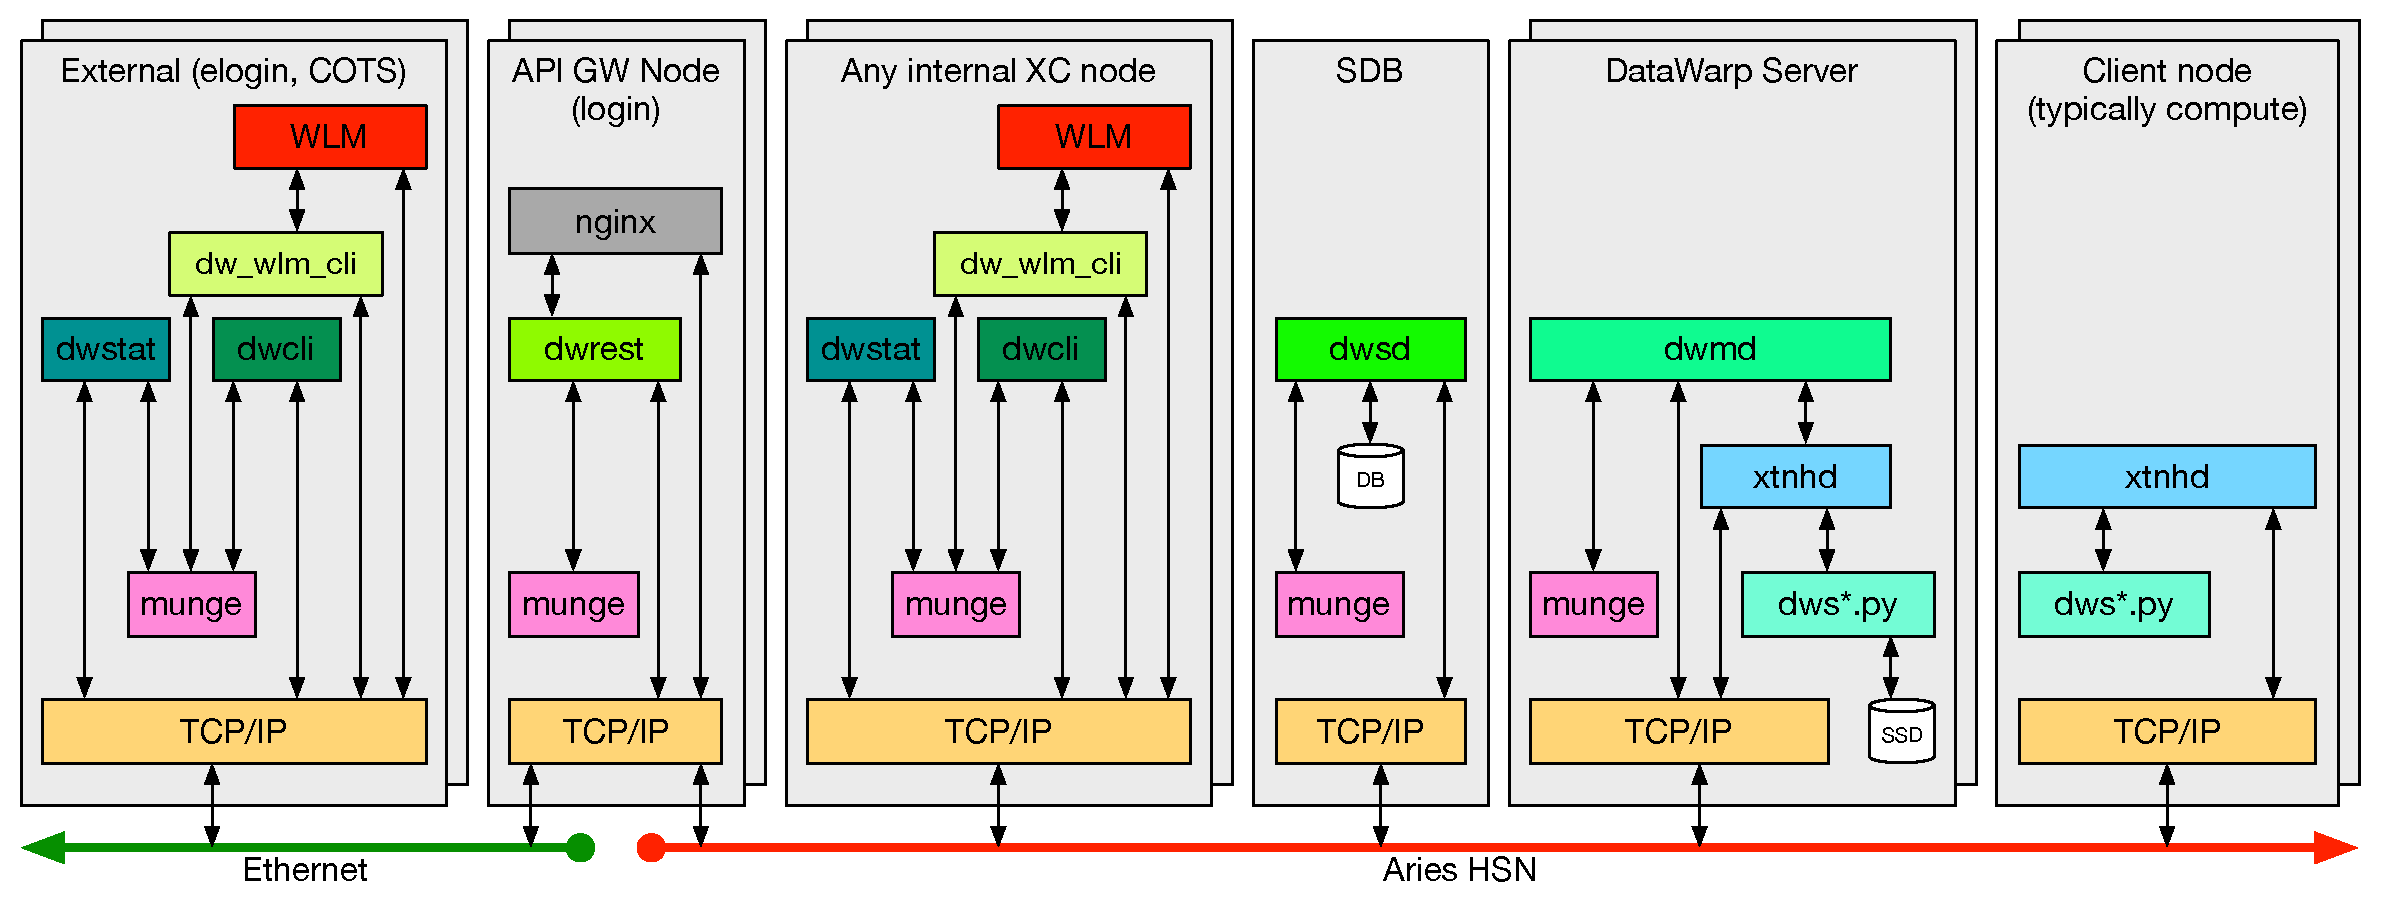
\includegraphics[width=\textwidth]{graphics/orchestration}
\caption{Visual overview of the components involved with orchestration.  For transparent caching, modifications were required for \texttt{dw\_wlm\_cli}, \texttt{dwstat}, \texttt{dwcli}, \texttt{dwrest}, \texttt{dwsd}, \texttt{dwmd}, and \texttt{dws*.py} scripts .\label{orchestration}}
\end{figure*}

For transparent cache, no additional support is required from a WLM that already supports DataWarp with scratch configurations.  This is because the WLM's interest involves the capacity portion of a user's request and not the way in which the capacity is to be configured.  This intentional separation between DataWarp and WLM allows for new data paths to be introduced in to DataWarp with less work and coordination.  Similarly, the environment variable needed by users to locate the transparent cache mount is supplied to the WLM in the same way as the scratch environment variables.  The actual parsing of \texttt{\#DW} is handled by changes to the \texttt{dw\_wlm\_cli} client.

The DWS has three main responsibilities for transparent cache.  The timing of each specific step is controlled by callouts from the WLM.  The first of these is the set up of the transparent cache data path.  When setting up the data path, sub-steps tend to be blocked from starting on any node until prior sub-steps have completed on all nodes, e.g., mount points on compute nodes are not created until all servers have been successfully configured.  The \texttt{dwsd} daemon manages the scheduling of those steps, and sends messages to \texttt{dwmd} to perform them.  As with scratch, transparent cache environments are built upon DataWarp instances, which are allocations of SSD space across one or more DataWarp servers.  On each allocation fragment, the DWS makes an \texttt{XFS} filesystem.  This is used by the DataWarp filesystem components, \texttt{dcfs} and \texttt{dwfs}, to store file data.  The DWS creates the \texttt{dcfs} mount points, via changes to one of the \texttt{dws*.py} scripts, and specifies the \texttt{XFS} mount as the device and the user-requested PFS path as a mount option.  The DWS then creates a \texttt{dwfs} mount point and specifies the \texttt{dcfs} mount as the device, and the list of other servers in the allocation as a mount option.  The last step on each of the DataWarp servers is to create a namespace that is configured to span each server in the allocation.  The metadata directory specified at namespace creation time is a bind mount of the parallel filesystem directory which means many metadata operations actually rely on the PFS directly.  The DWS sets up the namespace via a library call that sends an \texttt{ioctl()} to \texttt{dwfs}.  In the final step for setup, the DWS makes a DVS mount on the nodes communicated to it by the WLM, i.e., the batch job's compute nodes.  At mount time, the device is supplied as the path corresponding to the remote nodes' namespace metadata directory, and the remote nodes in the instance are supplied as well.

The second responsibility the DWS has for transparent cache is managing dirty data in the cache prior to teardown.  Generally, any dirty data in the transparent cache environment should be allowed to be written back to the PFS prior to teardown taking place.  This is the default behavior.  There are cases where the dirty data may not need to be preserved, such as a failure in the compute job or a permanent partial failure of the DataWarp instance.  As with scratch, when there is interest in saving dirty data, the DWS, or \texttt{dwsd} specifically, will not allow the data path to be completely torn down until it has confirmation from it that the data has been successfully preserved.  For transparent cache, prior to removing a \texttt{dwfs} namespace the DWS will call in to the filesystem by having \texttt{dwsd} dispatch a request to \texttt{dwmd}, which will invoke a \texttt{dws*.py} script, which will use an \texttt{ioctl()} targeting \texttt{dcfs} designed to both initiate write-back of any dirty data and block returning until success or error.  On error, the message is logged and the operation retried after a short period of time.

The third responsibility the DWS has for transparent cache is teardown of the data path.  Generally, teardown takes place in reverse order from that of setup.  The DVS mount points on all compute nodes are unmounted first.  Then, the previously mentioned dirty data management step takes place.  It is crucial that the DVS mount points were removed first because dirty data could have been in a DVS client-side cache, or in transit between the compute nodes and DataWarp nodes.  After all dirty data has been written back to the PFS or the DWS has been instructed to skip this step, server teardown steps take place.  The DWS removes the namespaces on each server via a library call that sends an \texttt{ioctl()} to \texttt{dwfs}.  It then removes the bind mount of the PFS used during namespace setup.  The DWS then unmounts the \texttt{dwfs}, \texttt{dcfs}, and \texttt{XFS} filesystems, in that order.  The DWS then performs instance removal steps as it does with the scratch filesystem.

\section{Challenges\label{sec_chal}}

We faced a number of challenges in developing transparent caching.  Our first implementation of the data path did not re-use the \texttt{dwfs} component used in the scratch filesystem.  Instead, all the responsibilities of \texttt{dwfs} and \texttt{dcfs} were contained in a single filesystem layer, dwcfs or DataWarp Caching Filesystem.  This led to several problems such as higher maintenance costs and higher development costs.  By splitting the intra-node responsibilities (\texttt{dcfs}) from the inter-node responsibilities (\texttt{dwfs}) we were able to reduce both of these costs.  Having a more modular solution also reduced the learning curve associated with working on the implementation.

Just prior to the first release of transparent caching we realized that the orchestration layer would allow users to transparently cache directories that PFS filesystem permissions would otherwise suggest the user could not access.  For example, when interacting with a file path on a PFS, it is necessary to have execute permissions on all parent directories.  Since the orchestration layer originally allowed a user to supply any PFS path, and the orchestration layer would then bind mount that path on to a \texttt{dwfs} namespace tree as root, the parent directory permissions were effectively ignored.  To handle this problem, administrators can now configure the DWS to be more restrictive when processing transparent cache configuration requests.

Since the transparent cache data path relies on the PFS for metadata operations, it generally does not accelerate them.  Since these operations must route through DVS in addition to through the PFS, the extra overhead can even result in decreased metadata performance.  We are considering improvements to DVS to reduce this overhead.  Since the number of PFS clients in a transparent cache data path is the number of DataWarp servers rather than the number of compute nodes, it is possible to get better metadata performance.  For large jobs where the compute node count is larger than the number of DataWarp servers, the fewer PFS clients means less coordination is required overall.

Throughout the course of development and testing we ran in to bugs that needed to be triaged and fixed.  What made this trickier was running in to PFS bugs.  In particular for lustre we found issues involving group lock functionality and open by handle functionality (proof read this).  Collaborating with lustre experts was critical in understanding and making progress on these issues.

Implementing recovery of transparent caching filesystems on server crash or reboot has also proven challenging, and is not present in the current implementation.  We have found bugs in how XFS manages sparse files that prevent us from using it during recovery.  While the bugs are fixed in newer Linux releases, the fixes are not easily back-ported to current CLE releases.

\section{Early Experience\label{sec_ee}}

Implementation of Transparent Cache DataWarp (TC) for the NERSC user environment was of particular interest due to the wide range of user skill set and breadth of applications deployed on the XC40 (Cori).  DataWarp usage had been well accepted by users, was stable and performant.  It did however require a bit of forethought to determine input and output file requirements (names, location, size) for staging and allocation size directives.  The Transparent Cache \texttt{\#DW} directives simplifies the implementation for less technical users while still providing improved filesystem performance.

Cray's development of Transparent Cache was still ongoing and was not yet a released product that could be installed without risk of destabilizing the production system (Cori). Like many sites, NERSC maintains a TDS for each of the main production systems (Test and Development System).  The initial installation was then targeted for the TDS.  The TDS (Gerty) has a minimalistic DataWarp configuration comprising two DW-servers with 12TB of SSD.  The software revisions on  the TDS mirror those of the main system.

The primary purpose of the TDS is to support the installation of new OS releases or patch sets prior to roll out onto Cori.  The installation of the pre-release of Transparent Cache would render this functionality ineffective due to the differences in the software levels and code differences (for example DVS). Therefore a plan was developed where both purposes could be served.  A snapshot of the TDS' current SMW filesystem (BTRFS) containing the base configuration sets (cfgsets) and images (P0 images) would be created to revert back to. The TC filesets were then applied to the TDS, images generated for each type of node and another BTRFS snapshot taken.  This would allow switching between snapshots, selecting which node image to boot (cnode update), and booting the TDS in either 'normal mode' or 'TC mode'.  Management and coordination of this activity is aided by a 'gitflow'-like environment as detailed in "Managing the SMW as a git Branch" - CUG2018 Jacobsen/Kleinman/Longley~\cite{cug_git_smw}. 

After rebooting the TDS with the TC-images the DWS configuration had to be restored from a JSON backup due to the change in revision levels.  This involved two simple steps, one before updating and one after- using the "dwcli config" command with:
\begin{enumerate}
\item \textbf{backup} - backup node/pool configuration to stdout (json)
\item \textbf{restore} - attempt to restore a previously saved configuration from stdin (json)
\end{enumerate}

For our initial performance testing we used two plasma physics applications; \texttt{VPIC} (writing output to a single file using the HDF5 interface) and \texttt{BD-CATS} (Big Data Clustering at Trillion Particle Scale cosmology) as shown in \figurename~\ref{vpic}.  The performance returned from Transparent Cache indicates a speed up of 1.5 to 2.2 times that of the Lustre filesystem.

\begin{figure*}
\centering
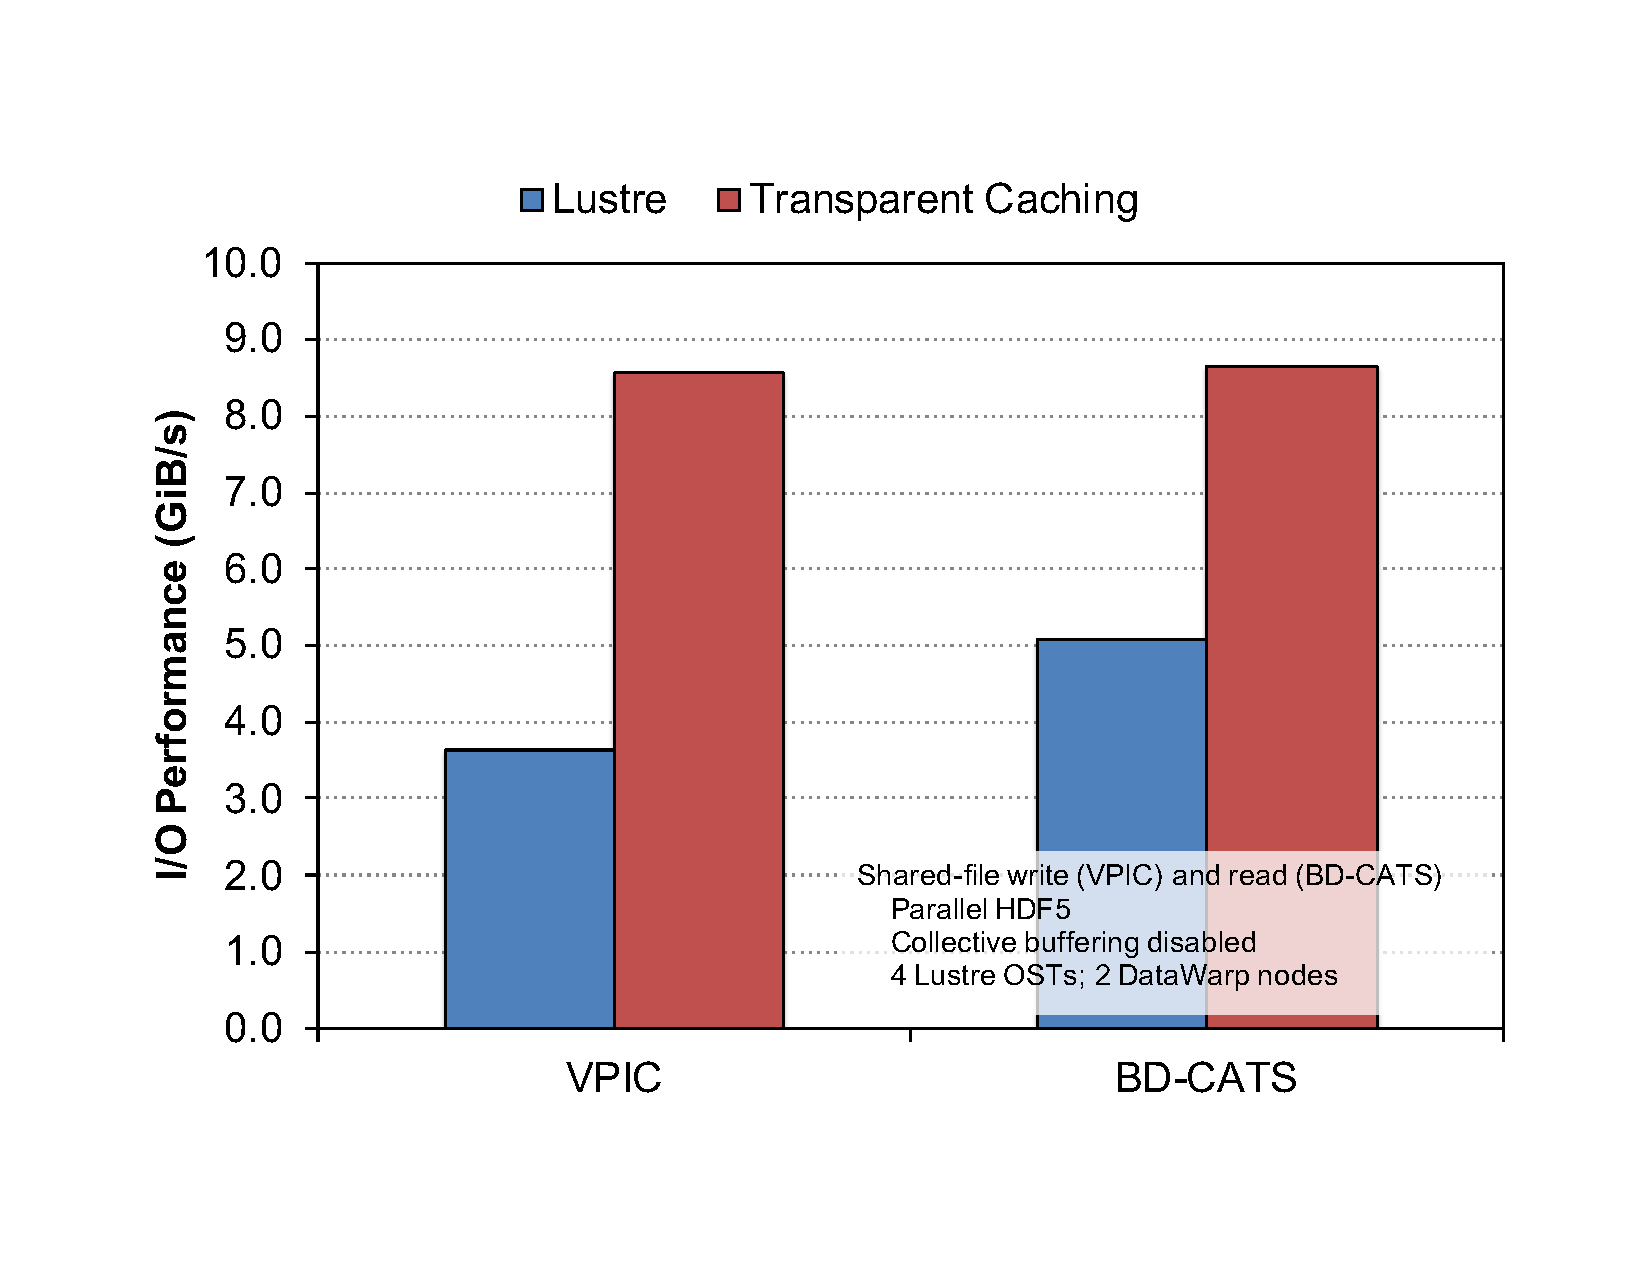
\includegraphics[width=\textwidth]{graphics/vpic}
\caption{Initial performance results with \texttt{VPIC} and \texttt{BD-CATS}. Courtesy Glenn Lockwood, NERSC.\label{vpic}}
\end{figure*}

\section{Future Work\label{sec_fw}}

Load balance access mode for transparent caching is meant to greatly accelerate read-only workloads.  While the old transparent caching data path implementation supported this access mode, the new implementation does not yet do so.  Rather than striping files across all DataWarp servers as in striped access mode, with load balance access mode files are duplicated on each DataWarp server.  Then, each compute node forwards all IO requests to just one of the DataWarp nodes.  When many ranks all need to read the same file simultaneously, the full bandwidth from all servers is used immediately.

While transparent caching does automatically copy up data from the PFS in to the transparent cache on demand, it can still be useful to preload the cache before a batch job starts.  This is similar to the scratch data path environment, where files can be staged (copied) on to the SSDs prior to when a batch job script executes.  For batch job scripts that start out reading a large input file such as a checkpoint or database, copying up the file in to the cache beforehand is beneficial.  We envision this as new batch job script directive, \texttt{\#DW preload}.

Similarly, while transparent caching does automatically manage the contents of the cache, if given hints by a user it can perform better.  By allowing users to explicitly request copy-up, eviction, write-back, or invalidation, the cache hit ratio can be improved and batch job execution time can be decreased.

The thresholds used by the current transparent caching eviction and write-back algorithms are preliminary and not optimal for all batch jobs.  With more experience and empirical data, we will change these thresholds to be better for jobs on average, and allow for per-job configuration of these values.

The old transparent caching implementation exposed statistics or accounting data via a C library API, but the new implementation does not expose this information.  The data is useful in seeing how effectively the transparent cache operated, such as seeing the cache hit ratio.  The information can be used to inform increasing or decreasing the size of the transparent cache environment.

The default behavior for \texttt{close()} and \texttt{fsync()}-like operations in transparent caching is to sync all dirty data to the SSDs.  Allowing this behavior to be configurable, e.g., so that all dirty data is guaranteed to have been written to the PFS on successful completion, will allow for users to choose between speed of operation and having a simple method for guaranteeing durability of data.

\section{Conclusion\label{sec_conc}}
Cray's Datawarp BurstBuffer provides a scalable, highly performant I/O system for the challenges of science at scale.  Technically capable scientists can take full advantage of the raw performance delivered with a few carefully placed directives.  For those scientists that are not technically savvy the implementation of Transparent Cache allows them to implement most of the performance advantages easily into their scientific workflows without having to worry the details of specific stage-in and stage-out of their datasets.  As development of TC continues and its performance tuned the users will 'transparently' benefit without changes to their code or job workflow scripts.

% use section* for acknowledgment
\ifCLASSOPTIONcompsoc
  % The Computer Society usually uses the plural form
  \section*{Acknowledgments}
\else
  % regular IEEE prefers the singular form
  \section*{Acknowledgment}
\fi

The authors would like to thank their teams and users at NERSC and Cray as well as those working in support of DataWarp at Adaptive, Altair, and SchedMD.





% trigger a \newpage just before the given reference
% number - used to balance the columns on the last page
% adjust value as needed - may need to be readjusted if
% the document is modified later
%\IEEEtriggeratref{8}
% The "triggered" command can be changed if desired:
%\IEEEtriggercmd{\enlargethispage{-5in}}

% references section

% can use a bibliography generated by BibTeX as a .bbl file
% BibTeX documentation can be easily obtained at:
% http://mirror.ctan.org/biblio/bibtex/contrib/doc/
% The IEEEtran BibTeX style support page is at:
% http://www.michaelshell.org/tex/ieeetran/bibtex/
\bibliographystyle{IEEEtran}
% argument is your BibTeX string definitions and bibliography database(s)
\bibliography{IEEEabrv,sources}
%
% <OR> manually copy in the resultant .bbl file
% set second argument of \begin to the number of references
% (used to reserve space for the reference number labels box)

% that's all folks
\end{document}


